% The deck in the README's screenshot.
\documentclass[aspectratio=169]{beamer}
\usetheme{moloch}
\usepackage{tikz}
\usetikzlibrary{arrows.meta,positioning,calc}

\title{The Knapsack Problem}
\subtitle{A five-minute tour}
\date{}

\begin{document}

\maketitle

\begin{frame}{The problem}
  Given $n$ items, item $i$ with value $v_i$ and weight $w_i$,
  and a knapsack of capacity $C$:
  \[
    \max \Big\{ \sum_{i=1}^{n} v_i x_i \;:\;
    \sum_{i=1}^{n} w_i x_i \le C,\; x \in \{0,1\}^n \Big\}
  \]
  \begin{itemize}
  \item NP-hard, yet solved in $O(nC)$ by dynamic programming.
  \item Its LP relaxation is solved greedily, by $v_i / w_i$.
  \end{itemize}
\end{frame}

\begin{frame}{Dynamic programming}
  $f_k(c)$: the best value with the first $k$ items and capacity $c$.
  \[
    f_k(c) = \max\{\, f_{k-1}(c),\; f_{k-1}(c - w_k) + v_k \,\}
  \]
  \begin{center}
  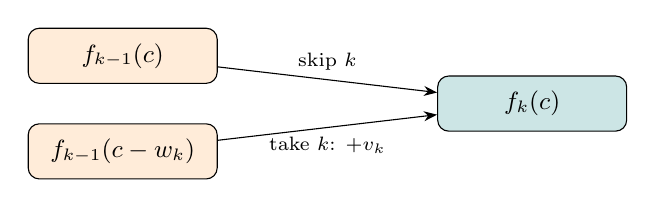
\begin{tikzpicture}[node distance=5mm and 22mm,
      s/.style={rectangle, rounded corners, draw, fill=orange!15,
                minimum height=7mm, minimum width=24mm, font=\small},
      >={Stealth}]
    \node[s] (a) {$f_{k-1}(c)$};
    \node[s, below=of a] (b) {$f_{k-1}(c-w_k)$};
    \node[s, fill=teal!20] (c) at ($(a)!0.5!(b) + (5.2,0)$) {$f_k(c)$};
    \draw[->] (a) -- node[above, font=\scriptsize] {skip $k$} (c);
    \draw[->] (b) -- node[below, font=\scriptsize] {take $k$: $+v_k$} (c);
  \end{tikzpicture}
  \end{center}
\end{frame}

\begin{frame}{Greedy bound}
  Sort by $v_1/w_1 \ge v_2/w_2 \ge \dots$ and fill until item $s$ no longer fits:
  \[
    U = \sum_{i<s} v_i + \frac{v_s}{w_s}\Big(C - \sum_{i<s} w_i\Big)
  \]
  \begin{block}{Dantzig's bound}
    $U$ is the LP optimum: an upper bound for branch and bound.
  \end{block}
\end{frame}

\end{document}
